% Options for packages loaded elsewhere
\PassOptionsToPackage{unicode}{hyperref}
\PassOptionsToPackage{hyphens}{url}
\PassOptionsToPackage{dvipsnames,svgnames*,x11names*}{xcolor}
%
\documentclass[
  ignorenonframetext,
  aspectratio=169]{beamer}
\usepackage{pgfpages}
\setbeamertemplate{caption}[numbered]
\setbeamertemplate{caption label separator}{: }
\setbeamercolor{caption name}{fg=normal text.fg}
\beamertemplatenavigationsymbolsempty
% Prevent slide breaks in the middle of a paragraph
\widowpenalties 1 10000
\raggedbottom
\setbeamertemplate{part page}{
  \centering
  \begin{beamercolorbox}[sep=16pt,center]{part title}
    \usebeamerfont{part title}\insertpart\par
  \end{beamercolorbox}
}
\setbeamertemplate{section page}{
  \centering
  \begin{beamercolorbox}[sep=12pt,center]{part title}
    \usebeamerfont{section title}\insertsection\par
  \end{beamercolorbox}
}
\setbeamertemplate{subsection page}{
  \centering
  \begin{beamercolorbox}[sep=8pt,center]{part title}
    \usebeamerfont{subsection title}\insertsubsection\par
  \end{beamercolorbox}
}
\AtBeginPart{
  \frame{\partpage}
}
\AtBeginSection{
  \ifbibliography
  \else
    \frame{\sectionpage}
  \fi
}
\AtBeginSubsection{
  \frame{\subsectionpage}
}
\usepackage{lmodern}
\usepackage{amssymb,amsmath}
\usepackage{ifxetex,ifluatex}
\ifnum 0\ifxetex 1\fi\ifluatex 1\fi=0 % if pdftex
  \usepackage[T1]{fontenc}
  \usepackage[utf8]{inputenc}
  \usepackage{textcomp} % provide euro and other symbols
\else % if luatex or xetex
  \usepackage{unicode-math}
  \defaultfontfeatures{Scale=MatchLowercase}
  \defaultfontfeatures[\rmfamily]{Ligatures=TeX,Scale=1}
\fi
\usetheme[]{Frankfurt}
\usecolortheme{beaver}
\usefonttheme{structuresmallcapsserif}
% Use upquote if available, for straight quotes in verbatim environments
\IfFileExists{upquote.sty}{\usepackage{upquote}}{}
\IfFileExists{microtype.sty}{% use microtype if available
  \usepackage[]{microtype}
  \UseMicrotypeSet[protrusion]{basicmath} % disable protrusion for tt fonts
}{}
\makeatletter
\@ifundefined{KOMAClassName}{% if non-KOMA class
  \IfFileExists{parskip.sty}{%
    \usepackage{parskip}
  }{% else
    \setlength{\parindent}{0pt}
    \setlength{\parskip}{6pt plus 2pt minus 1pt}}
}{% if KOMA class
  \KOMAoptions{parskip=half}}
\makeatother
\usepackage{xcolor}
\IfFileExists{xurl.sty}{\usepackage{xurl}}{} % add URL line breaks if available
\IfFileExists{bookmark.sty}{\usepackage{bookmark}}{\usepackage{hyperref}}
\hypersetup{
  pdftitle={Molecular Markers and Marker Assisted Selection},
  pdfauthor={Deependra Dhakal},
  colorlinks=true,
  linkcolor=red,
  filecolor=Maroon,
  citecolor=blue,
  urlcolor=red,
  pdfcreator={LaTeX via pandoc}}
\urlstyle{same} % disable monospaced font for URLs
\newif\ifbibliography
\setlength{\emergencystretch}{3em} % prevent overfull lines
\providecommand{\tightlist}{%
  \setlength{\itemsep}{0pt}\setlength{\parskip}{0pt}}
\setcounter{secnumdepth}{-\maxdimen} % remove section numbering
\usepackage{booktabs}
\usepackage{longtable}
\usepackage{array}
\usepackage{multirow}
\usepackage{wrapfig}
\usepackage{float}
\usepackage{colortbl}
\usepackage{pdflscape}
\usepackage{tabu}
\usepackage{threeparttable}
\usepackage{threeparttablex}
\usepackage[normalem]{ulem}
\usepackage{makecell}
\usepackage{xcolor}

% % set background image if you will
% \usebackgroundtemplate%
% {%
%     \includegraphics[width=\paperwidth,height=\paperheight]{02-dna_modification_background_dna_helix.jpg}%
% }

% % set background in a TikZ node for modifications
% % set background in a TikZ node for modifications
\usepackage{tikz}
\usepackage[absolute,overlay]{textpos}
% \setlength{\TPHorizModule}{\textwidth}
% \setlength{\TPVertModule}{\textheight}

\setbeamertemplate{title page}{
\tikz\node[opacity=0.8] {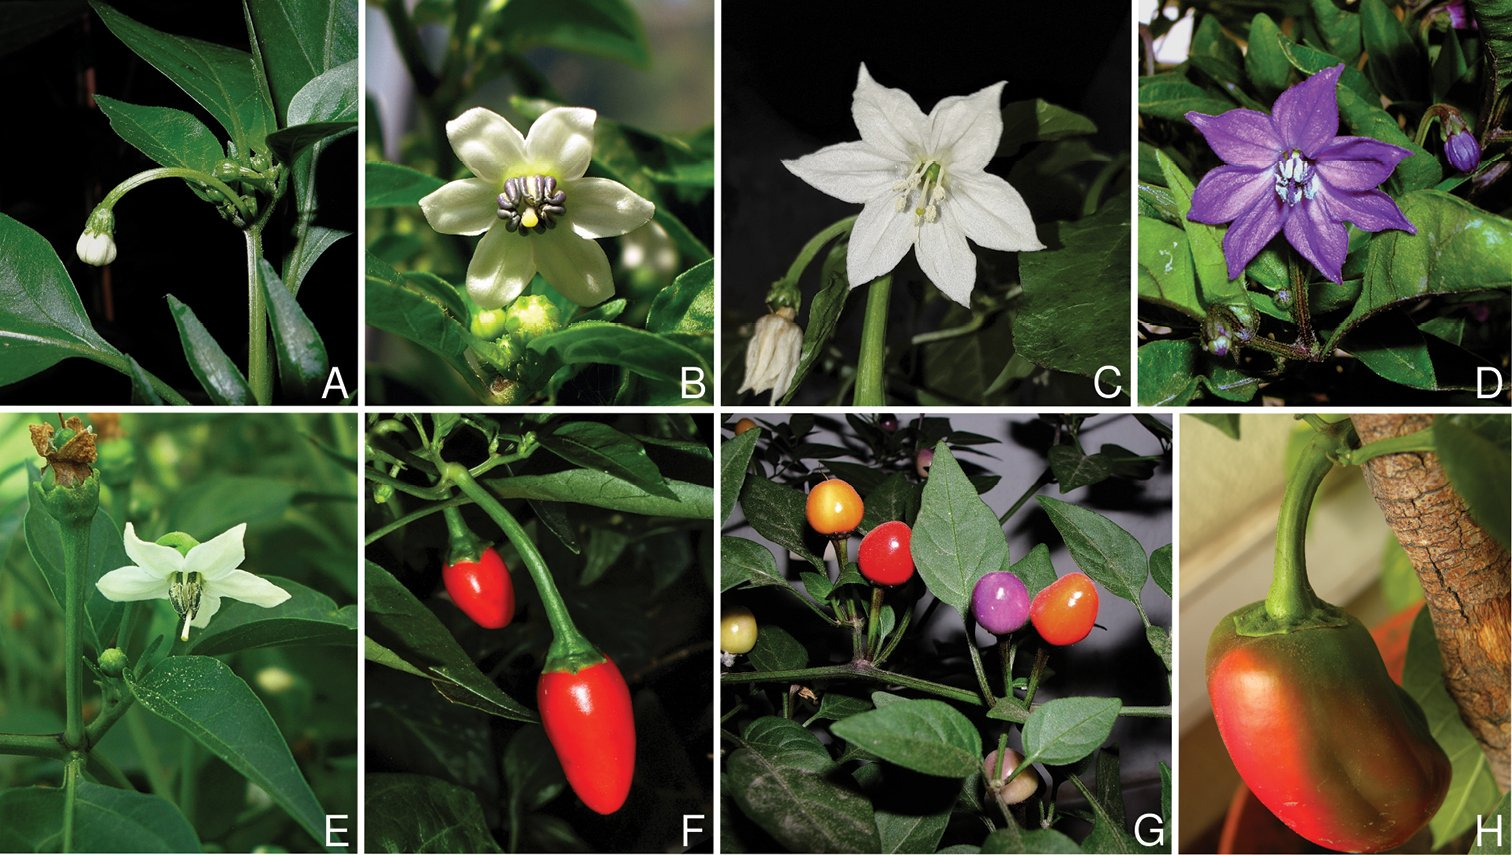
\includegraphics[width=0.8\paperwidth]{./07-molecular_markers_chilli_cover.jpeg}};
% \tikz\node[opacity=0.8] {\includegraphics[width=5cm,ext=.1-overview_mutation_cover.png,type=png,read=.1-overview_mutation_cover.png]{1}} % if name shall contain dots, suppose filename = 01.1-overview_mutation_cover.png
\begin{textblock}{15}(3.5,6)\usebeamerfont{title} % whole page is layed in a grid of 15x15 relative units and text is written starting from the coordinates layed in parens (horizontal=3.5,vertical=6)
{\color{white}\raggedright\par\inserttitle}\\[0.4cm]
{\color{white}\raggedright{\insertauthor}\mbox{}\\[0.2cm]
\insertdate}
\end{textblock}} % dd_rookie modified, figure is top aligned

% % set caption font size
% % note that beamer presentation native captions have their own configs
% \usepackage{caption}
% \captionsetup{font=footnotesize}

% this font option is amenable for beamer
\setbeamerfont{caption}{size=\tiny}

% some beamer themes naturally might not support navigation symbols
% \setbeamertemplate{navigation symbols}{} % remove navigation symbols

\setbeamertemplate{footline}[page number] % insert page number in footline

% \setbeamertemplate{navigation symbols}{slide} % insert slide indication in navigation
% \setbeamertemplate{navigation symbols}{frame} % insert frame indication in navigation
% \setbeamertemplate{navigation symbols}{section} % insert section indication in navigation
% \setbeamertemplate{navigation symbols}{subsection} % insert subsection indication in navigation

% \AtBeginSubsection{} % supress subsection display

\title{Molecular Markers and Marker Assisted Selection}
\subtitle{Molecular markers, MAS, Mapping strategy and Applications}
\author{Deependra Dhakal}
\date{Academic year: 2022-2023}
\institute{College of Natural Resource Management, Tikapur \and AFU}

\begin{document}
\frame{\titlepage}

\begin{frame}[allowframebreaks]
  \tableofcontents[hideallsubsections]
\end{frame}
\hypertarget{molecular-markers}{%
\section{Molecular markers}\label{molecular-markers}}

\begin{frame}{Definition and general features}
\protect\hypertarget{definition-and-general-features}{}
\begin{figure}

{\centering 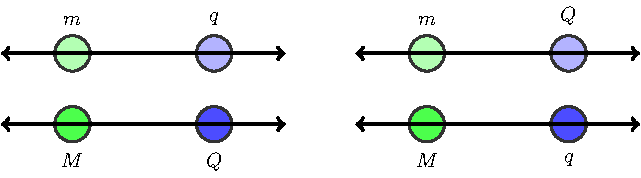
\includegraphics[width=0.9\linewidth]{../scripts/marker-qtl-association-diagram} 

}

\caption{Marker-QTL linkage for arbitray loci $Q$ and $M$. On the right, linked loci show $cis$-conformation, while those on the right show $trans$-conformation.}\label{fig:marker-trait-linkage}
\end{figure}
\end{frame}

\begin{frame}{Types}
\protect\hypertarget{types}{}
\footnotesize

\begin{itemize}
\tightlist
\item
  Genomic markers, have particular strengths and weakness, so,
  consideration and knowledge of the markers is necessary before use.
\item
  For instance, a RAPD marker is dominant (identifying only one band of
  distinction) and it may be sensitive to reproducible results. This is
  typically due to the conditions in which it was produced. RAPD's are
  used also under the assumption that two samples share a same locus
  when a sample is produced.
\item
  Commonly used molecular markers:

  \begin{itemize}
  \tightlist
  \item
    Restriction Fragment Length Polymorphism -- RFLP
  \item
    Random Amplified Polymorphic DNA -- RAPD
  \item
    Amplified Fragment Length Polymorphism -- AFLP
  \item
    Variable Number Tandem Repeat -- VNTR
  \item
    Oligonucleotide Polymorphism -- OP
  \item
    Single Nucleotide Polymorphism -- SNP
  \item
    Allele Specific Associated Primers -- ASAP
  \item
    Inverse Sequence-tagged Repeats -- ISTR
  \end{itemize}
\end{itemize}
\end{frame}

\begin{frame}{Applications}
\protect\hypertarget{applications}{}
\begin{itemize}
\tightlist
\item
  Assessing variability of genetic differences and characteristics
  within a species.
\item
  Identification and fingerprinting of genotypes.
\item
  Estimating genetic distances between species and offspring.
\item
  Identifying location of QTLs.
\item
  Identification of DNA sequence from useful candidate genes.
\end{itemize}
\end{frame}

\hypertarget{qtl-mapping}{%
\section{QTL mapping}\label{qtl-mapping}}

\begin{frame}{Overview}
\protect\hypertarget{overview}{}
\begin{columns}[T,onlytextwidth]
  \column{0.6\textwidth}
  \footnotesize
  \begin{itemize}
  \item Genes that control variation in quantitative (or complex traits) are known as Quantitative Trait Loci (QTL) -- like genes!
  \item QTL have allelic variants that typically make relatively small, quantitative contributions to phenotype.
  \item Contribution of the alleles to a QTL to the trait value can be observed by looking at the frequency distributions associated with each genotype at a QTL as shown in Figure \ref{fig:allele-freq-distribution}.
  \end{itemize}
  \column{0.4\textwidth}
  
\begin{figure}
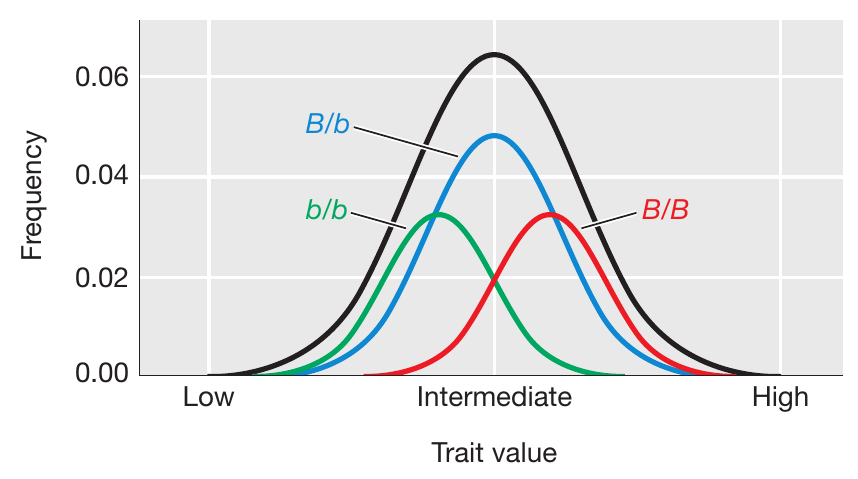
\includegraphics[width=0.9\linewidth]{../images/frequency_distribution_showing_contribution_qtl} \caption{Frequency distribution show the contributions of alleles at a QTL to a complex trait. Distributions for the different genotypic classes at QTL locus B relate to the overall distribution for the population (black lines)}\label{fig:allele-freq-distribution}
\end{figure}

\end{columns}
\end{frame}

\begin{frame}{Method}
\protect\hypertarget{method}{}
\footnotesize

\begin{itemize}
\tightlist
\item
  QTL mapping is based on idea that location of QTL in the genome can be
  identified using marker loci linked to a QTL.

  \begin{itemize}
  \tightlist
  \item
    Suppose you make a cross between two inbred strains -- P1 (with high
    trait value) and P2 (with low trait value).
  \item
    The F1 can be backcrossed to P1 to create a BC1 population in which
    the alleles at all the genes in the two parental genomes will
    segregate.
  \item
    Marker loci such as SNP or microsatellites can be scored
    unambiguously as homozygous P1 or heterozygous for each BC1
    individual.
  \item
    If there is a QTL linked to the marker locus, then the mean trait
    value for individuals that are homozygous P1 at the marker locus
    will be different from the mean trait value for the heterozygous
    individual.
  \end{itemize}
\end{itemize}
\end{frame}

\begin{frame}{Example}
\protect\hypertarget{example}{}
\begin{figure}
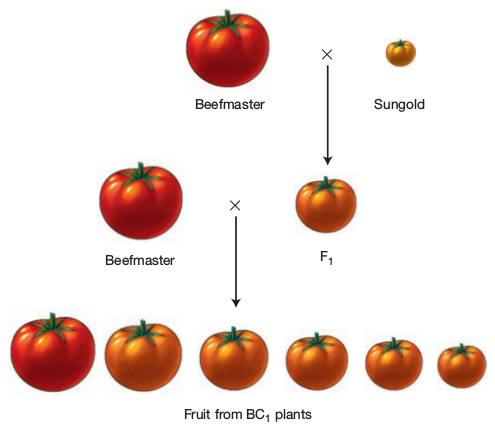
\includegraphics[width=0.3\linewidth]{../images/tomato-beefmaster-sungold-cross} \caption{Breeding scheme for a BC population between Beefmaster and Sunglod tomatoes. In the BC1 generation, there is a continuous range of fruit sizes.}\label{fig:tomato-beefmaster-sungold-cross}
\end{figure}
\end{frame}

\begin{frame}{}
\protect\hypertarget{section}{}
\begin{columns}[T,onlytextwidth]
  \column{0.4\textwidth}
  \begin{itemize}
  \footnotesize
  \item Let us take two inbred lines of tomato that differ in fruit weight -- Beefmaster with fruits of 230 g and Sungold with fruits of 10 g weights.
  \item Cross the two lines to produce F1, then backcross the F1 to the beefmaster line to produce BC1 generation.
  \item Several hundered BC1 plants are grown and their fruit weights measured.
  \item Extract DNA from each of the BC1 plants. These DNA samples are used to determine the genotype of each plant at a set of marker loci (SSRs) (~100)  that are distributed across all of the chromosomes such that we have marker locus every 5 to 10 centimorgans.
  \end{itemize}
  \column{0.6\textwidth}

\begin{figure}
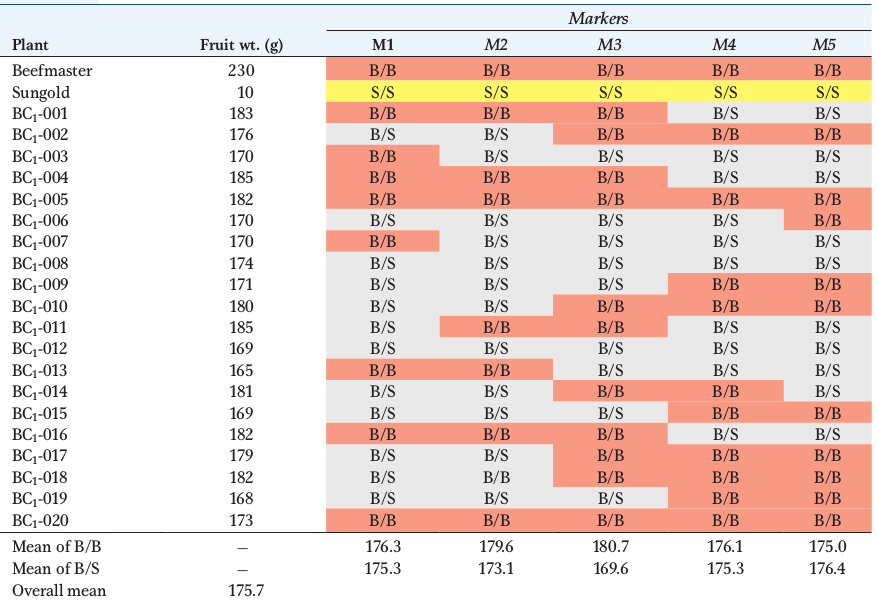
\includegraphics[width=0.95\linewidth]{../images/tomato-fruit-weight-marker-data} \caption{Example data of fruit weight and marker-locus data for BC population between inbred lines.}\label{fig:tomato-fruit-weight-marker-data}
\end{figure}

\end{columns}
\end{frame}

\begin{frame}{}
\protect\hypertarget{section-1}{}
\begin{itemize}
\tightlist
\item
  For each BC1 plant, we have the weight of its fruit and the genotypes
  at the marker loci. (Note: Trait values for the BC1 are intermediate
  between the two parents, but closer to the Beefmaster)
\item
  Since this is BC population, the genotypes at each marker locus is
  either B/B or B/S.
\item
  Crossover results in two markers appearing in recombinant/non-parental
  alignments (eg, BC1-001 has crossover between marker loci M3 and M4).
\item
  The expectation is that there is no QTL affecting fruit weight near M1
  -- For M1, the mean for genotypic classes B/B is 176.3 adn that for
  B/S is 175.3 (both lying close to overall mean 175.7). Now determine
  that for M3 ?
\item
  For M3, it matches the expectation that there is a QTL affecting fruit
  weight near M3.
\end{itemize}
\end{frame}

\hypertarget{marker-assisted-selection}{%
\section{Marker Assisted Selection}\label{marker-assisted-selection}}

\begin{frame}{Overview}
\protect\hypertarget{overview-1}{}
\begin{itemize}
\tightlist
\item
  Individual genes contributing to complex plant traits can sometimes be
  discovered through their association with genetic markers --
  \alert{QTL analysis}.
\item
  Use of molecular markers in detecting regions of genome and
  discriminating between genotypes based on genomic features that
  enhance chances of inheriting favorable quantitative trait loci is
  called MAS.
\item
  Rather than selecting traits, which are outcome of many genes, MAS is
  based on selecting specific alleles at marker loci that are known to
  be linked to the genes that cause the desired trait.
\end{itemize}
\end{frame}

\begin{frame}{Advantages}
\protect\hypertarget{advantages}{}
\begin{enumerate}
\tightlist
\item
  Avoids errors caused by environmental variance
\item
  Can be applied at a juvenile stage before a trait is expressed
\item
  Can be applied on a single plant
\item
  May be less expensive than phenotypic selection (it is debatable!)
\end{enumerate}

\begin{figure}
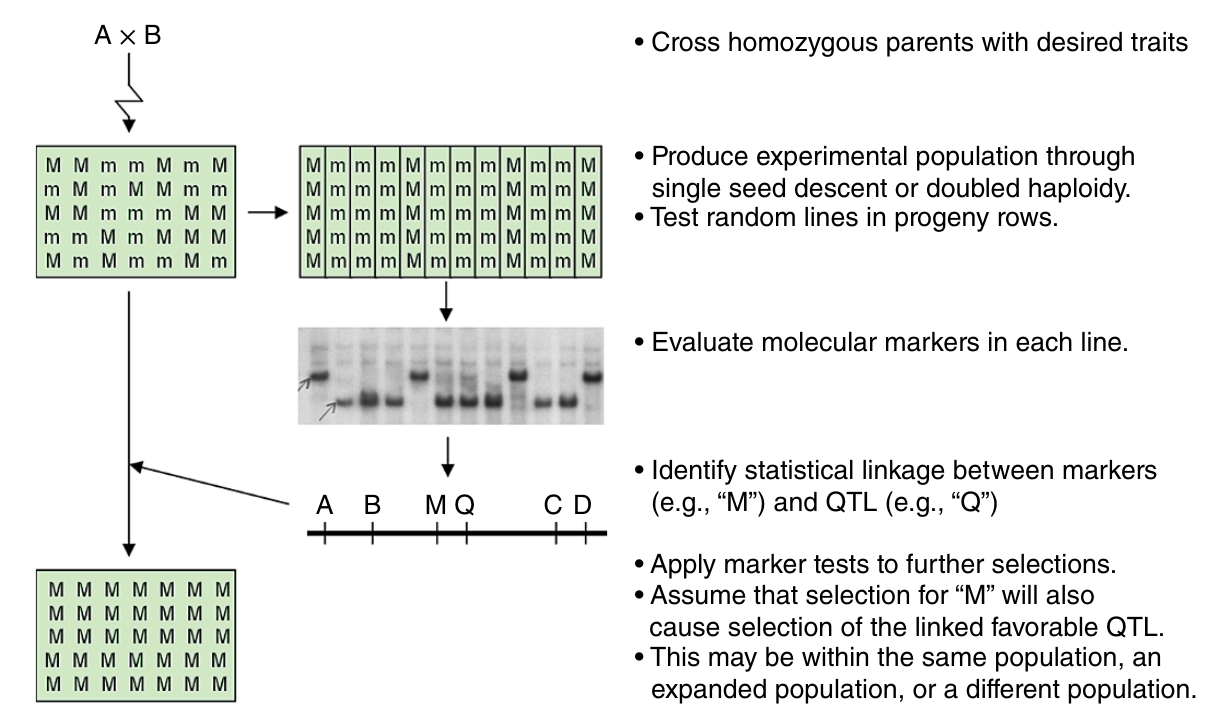
\includegraphics[width=0.38\linewidth]{../images/marker_assisted_selection} \caption{A simplified strategy for MAS. Here, a significant association between a QTL (Q) and a molecular marker allele (M) is identified in an experimental population. This information is applied in future populations in order to select Q indirectly through its linkage to M.}\label{fig:marker-assisted-selection}
\end{figure}
\end{frame}

\begin{frame}{Requirements of QTL mapping}
\protect\hypertarget{requirements-of-qtl-mapping}{}
\begin{itemize}
\tightlist
\item
  Breeding facilities with environmental control, accurate phenotyping
  and trained manpower
\item
  Incomplete linkage between a marker and the target QTL reduces the
  effectiveness of MAS
\item
  Marker must be polymorphic on the parents
\item
  MAS is effective only if the alleles being selected are important
  relative to other alleles in the population; For example a breeder
  might identify that allele A1 at locus A has a positive effect on
  yield. But this prediction would be made in a limited set of
  environments, and with a limited set of germplasm. A breeder who
  crossed a parent containing allele A1 with a new parent containing
  allele A4, and selected for A1 using a linked marker, might never
  discover that A4 is actually better than allele A1, or perhaps that
  allele A1 causes plants to be susceptible to a disease that was not
  present when A1 was first characterized. Hence, MAS should never to
  applied independently of phenotypic selection.
\end{itemize}
\end{frame}

\begin{frame}{Factors affecting QTL mapping using biparental
populations}
\protect\hypertarget{factors-affecting-qtl-mapping-using-biparental-populations}{}
\footnotesize

\begin{enumerate}
\tightlist
\item
  Size of mapping population
\end{enumerate}

\begin{itemize}
\tightlist
\item
  More the number of individuals in the population, more accurate the
  linkage map and accuracy in QTL results will be.
\item
  Chances of detecting QTL with minor effects is high with larger
  population size
\item
  Preferably \textgreater{} 200.
\item
  Lesser population \textasciitilde{} overestimated QTL effects.
\end{itemize}

\begin{enumerate}
\setcounter{enumi}{1}
\tightlist
\item
  Nature of mapping populations
\end{enumerate}

\begin{itemize}
\tightlist
\item
  Linkage maps could be drawn from the biparental populations in the
  following order of precision: F2 \textless{} BC \textless{} DH
  \(\leq\) RILs
\item
  Multiparental population such as Multi-parent Advanced Generation
  Intercross (MAGIC) populations, Nested Association Mapping (NAM)
  populations, Multiline Cross Inbred Line (MCILs), and Recombinant
  Inbred Advanced Intercross Lines (RIAILs) have to led to development
  of unique LD analysis methods and have variying accuracies.
\end{itemize}
\end{frame}

\begin{frame}{}
\protect\hypertarget{section-2}{}
\begin{enumerate}
\setcounter{enumi}{2}
\tightlist
\item
  Density and coverage of markers in the linkage map
\end{enumerate}

\begin{itemize}
\tightlist
\item
  More the markers on the map, less the interval distance between two
  markers and more accuracy in the results.
\end{itemize}

\begin{enumerate}
\setcounter{enumi}{3}
\tightlist
\item
  Statistical methods used
\end{enumerate}

\begin{itemize}
\tightlist
\item
  Single Marker Analysis (SMA) \(<\) Simple Interval Mapping (SIM) \(<\)
  Composite Interval Mapping (CIM) \(<\) Inclusive Compositve Interval
  Mapping (ICIM) \(\leq\) Bayesian Interval Mapping (BIM)
\end{itemize}
\end{frame}

\begin{frame}{}
\protect\hypertarget{section-3}{}
\begin{enumerate}
\setcounter{enumi}{4}
\tightlist
\item
  Heritability of the trait
\end{enumerate}

\begin{itemize}
\tightlist
\item
  Greater the \(h^2\), more the chance of QTL detection
\end{itemize}

\begin{enumerate}
\setcounter{enumi}{5}
\tightlist
\item
  Significance criteria used
\end{enumerate}

\begin{itemize}
\tightlist
\item
  More false positives with arbitrary significance criteria; robustness
  and accuracy increases with permutation test and threshold values.
\end{itemize}
\end{frame}

\begin{frame}{}
\protect\hypertarget{section-4}{}
\begin{enumerate}
\setcounter{enumi}{6}
\tightlist
\item
  Effect of environment
\end{enumerate}

\begin{itemize}
\tightlist
\item
  If the effect size of the QTL is small, it may not be detected in all
  the environments.
\end{itemize}

\begin{enumerate}
\setcounter{enumi}{7}
\tightlist
\item
  Experimental errors
\end{enumerate}

\begin{itemize}
\tightlist
\item
  Greater the precision of phenotyping, chances increase for detection
  of small effect QTLs;
\item
  Errors in scoring of genotypic data as well as missing marker data can
  affect the order of markers on the linkage map and can affect the
  estimated QTL location.
\end{itemize}
\end{frame}

\begin{frame}{Progress in MAS}
\protect\hypertarget{progress-in-mas}{}
\begin{itemize}
\tightlist
\item
  It is now possible to select across a genome rather than select for
  one or several markers for single QTLs. Genomic selection is an
  extension of MAS.
\item
  In soybean, 50,000 single nucleotide polymorphic (SNP) markers are now
  available for use by breeders.
\end{itemize}
\end{frame}

\hypertarget{bibliography}{%
\section{Bibliography}\label{bibliography}}

\begin{frame}{References}
\protect\hypertarget{references}{}
\end{frame}

\end{document}
